\section{Adding a dependency from Maven repository}

Maven repository stores all the artifacts that repository users have deployed, and we can take the advantage of Maven repository to add project dependencies on your other projects or other developers' projects. In this task, you are going to add a dependency of Stanford CoreNLP, which is hosted on the Central Repository. In the next homework, you will find several useful dependencies in our project repository.

\begin{enumerate}
 
\begin{figure}[t]
\centering
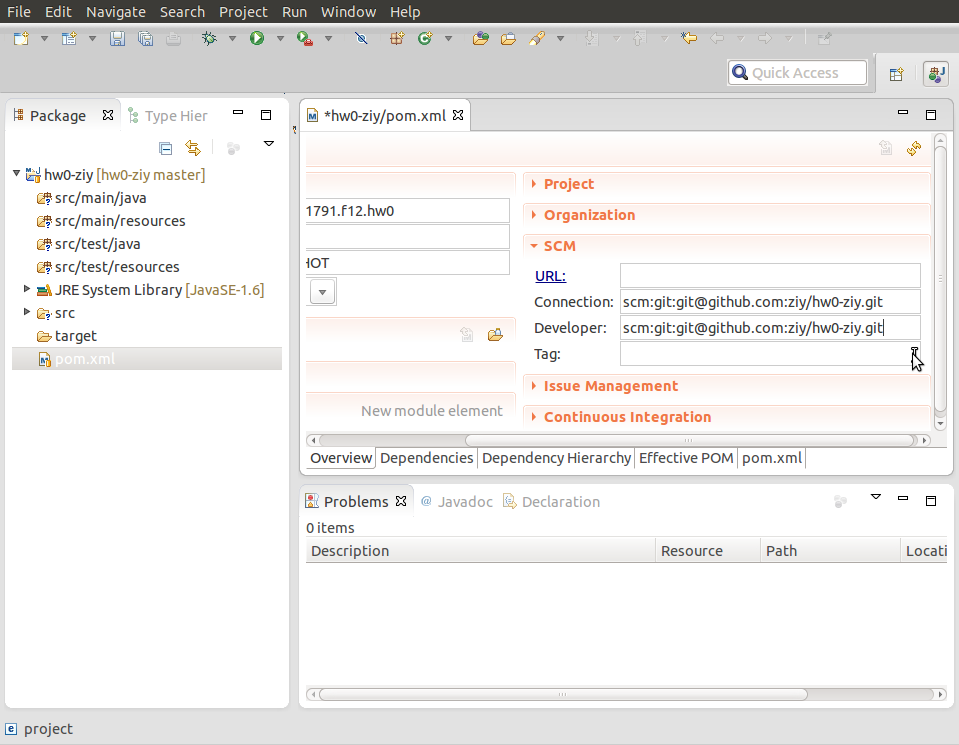
\includegraphics[scale=0.3]{repo-01-pom}
\caption{Opening a POM file\label{repo-01-pom}}
\end{figure}

\item Do you remember how the configuration of your Maven project is stored? Yes, the pom.xml file! Open it by double clicking the file name, and you will see the pom.xml is opened with ``Maven POM Editor'' as in Figure \ref{repo-01-pom}. If you find it is opened with a XML Editor or Text Editor, you should right click on the file name, you choose \textbf{Open With} $\rightarrow$ \textbf{Maven POM Editor}.
\item Before you add a dependency to your Maven project, you might want to look at all the tabs by clicking the tab name at the bottom of the Maven POM Editor. In the ``Overview'' tab, you need to type in some SCM information. Maven will use this information to connect to your remote GitHub repository. In general, the format of the scm is:

\begin{verbatim}
scm:<SCM_PROVIDER><DELIMITER><PROVIDER_SPECIFIC_PART>
\end{verbatim}

In particular to Git, most Git SCM providers could support two different URL syntaxes:

\begin{verbatim}
scm:git:git://SERVER_NAME/PATH_TO_REPOSITORY
\end{verbatim}

or specifically, 

\begin{verbatim}
scm:git:git://github.com/GITHUB_ID/REPOSITORY_ID.git
\end{verbatim}

and

\begin{verbatim}
scm:git:git@github.com:GITHUB_ID/REPOSITORY_ID.git
\end{verbatim}

You need to type in the SCM URL corresponding to your remote repository in \textbf{Connection} and \textbf{Developer} under \textbf{SCM} field. Details of SCM URL can be found at \url{http://maven.apache.org/scm/scm-url-format.html}.

\lstinputlisting[language=XML,float,linewidth=1.1\textwidth,caption=Configuring pom.xml,label=pom]{../lst/pom.xml}

\item Next, you should inform Maven what the URL of our course Maven repository is, which can be done by editing the POM file directly. Click the last tab ``pom.xml'', you are able to edit directly from the Maven POM Editor. Compare your POM content with Listing \ref{pom}, and add the missing lines to your POM.

As you've already specified the Group Id, Artifact Id, SCM information in early steps through the setup wizard or ``Overview'' tab of Maven POM Editor, you will find these concents (similar to Line 1 to 11 in Listing \ref{pom}) are already there to in you POM. You need to copy the content from Line 12 to Line 48 from Listing \ref{pom} into your POM. We will briefly describe what the meaning of each POM block is.

\begin{itemize}
\item[repositories] (Line 12 to 15) define a subset of your repositories (declared in your \verb|settings.xml| file) related to the current Maven project. You could retrieve all the existing artifacts from these repositories to make your current project depend on. Note that once you add a new \textbf{repository} item in the \textbf{repositories} group, you are enabled to view the artifacts in the ``Maven Repositories'' view (in next task).
\item[distributionManagement] (Line 16 to 25) will be used only if you plan to make a release for your artifact. For example, in Listing \ref{pom}, repositories for releases and snapshots are separately defined.
\item[plugins] (Line 26 to 46) include specific plug-ins required by the project to perform Maven goals. For example, you should specify the location of your pom.xml file when you perform the \verb|release:perform| goal.
\end{itemize}

\begin{qa}
\item[Q1] Is m2e so stupid? Part of the POM can be editted with perfect GUI or wizard, but why do we need to manually type in additional XML texts?
\item[A1] We are also able to add dependencies (in the next few steps) and add plugins into the pom.xml content with m2e GUI, but you have to add fields, such as \textbf{repositories}, \textbf{distributionManagement}, and so on, manually and directly to pom.xml, because the m2e plugin does not support add such fields in a more effect way from Maven POM Editor. Guess what it means? It means m2e does not recommend us to manually add these contents to pom.xml, although they are crucial to a Maven project.

Can you find the difference between the contents those can be added with GUI and those cannot? Contents added by GUI are usually project specific, while manually added contents are usually global contents shared across different projects in your workspace and organization, which means a ``meta'' pom should be generated for all the individual ``child'' Maven project. That's how Maven and archetype were originally introduced. We will learn to create a Maven project from an archetype in your next homework.
\end{qa}

\item Finally, try to press \textbf{Ctrl+Shift+F} within the pom.xml editor scope!

\begin{figure}[t]
\hspace{-1em}
\begin{minipage}{0.5\textwidth}
\centering
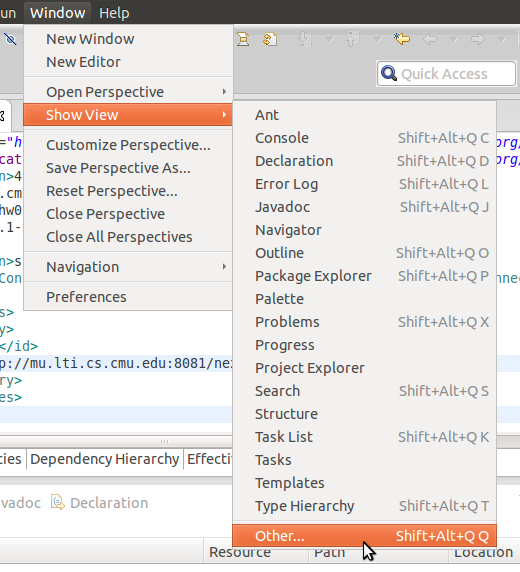
\includegraphics[scale=0.3]{repo-02-view}
\caption{Opening a new view\label{repo-02-view}}
\end{minipage}
\hfill
\begin{minipage}{0.5\textwidth}
\centering
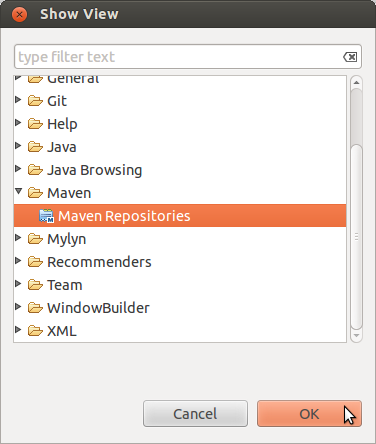
\includegraphics[scale=0.3]{repo-03-maven-repo}
\caption{Choosing Maven Repository view\label{repo-03-maven-repo}}
\end{minipage}
\hspace{-1em}
\end{figure}

\item Now click \textbf{Window} $\rightarrow$ \textbf{Show View} $\rightarrow$ \textbf{Other\ldots} to select a new view. See Figure \ref{repo-04-project-repo}.

\item In the ``Show View'' window, select \textbf{Maven} $\rightarrow$ \textbf{Maven Repositories} to open the ``Maven Repositories'' view. See Figure \ref{repo-05-dependency}.

\begin{figure}[t]
\centering
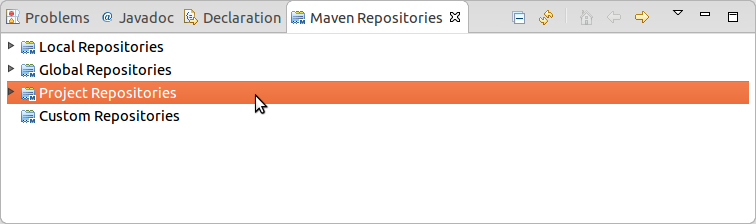
\includegraphics[scale=0.3]{repo-04-project-repo}
\caption{Viewing additional project repository from Maven Repository view\label{repo-04-project-repo}}
\end{figure}

\item You can see the ``Maven Repositories'' view at the bottom of your workspace, you are able to unfold ``Project Repositories'' since you have added items in the \textbf{repositories} field of your \verb|pom.xml| file.

\begin{qa}
\item[Q1] I could not unfold the \textbf{Project Repositories} or there is no artifact inside it.
\item[A1] You should try the following three solutions:

\begin{enumerate}
\item As you did before, go back to \textbf{Edit} (or \textbf{Window}) $\rightarrow$ \textbf{Preferences}, and choose \textbf{Maven} $\rightarrow$ \textbf{User Settings} again, you will see the plug-in could find the setting file you specified (see Figure \ref{eclipse-04-maven-setting-back}), and click \textbf{Update Settings}.
\item Click the ``double arrows'' icon (second icon in the top-right corner of ``Maven Repositories'' view) to reload settings.xml.
\item Right-click on each individual repository in ``Maven Repositories'' view (e.g. \textbf{deployment} in our example), select \textbf{Minimum Index Enabled} or \textbf{Enable Full Index} instead of \textbf{Disable Index Details}.
\end{enumerate}
\end{qa}

\begin{figure}[t]
\centering
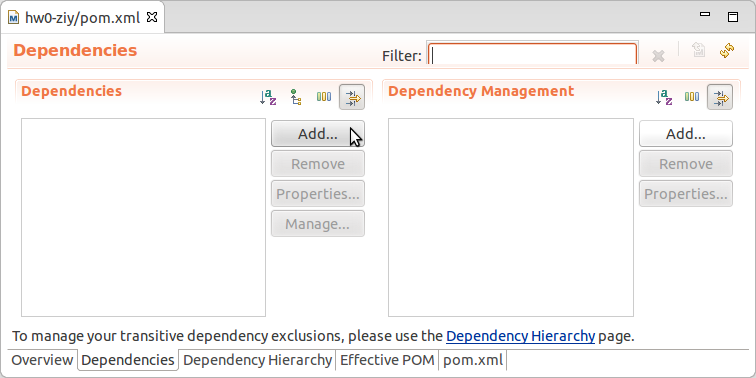
\includegraphics[scale=0.3]{repo-05-dependency}
\caption{Adding a Jar dependency\label{repo-05-dependency}}
\end{figure}

\item Now you could add an artifact dependency for your first Maven Project. Go to the \textbf{Dependencies} tab in Maven POM Editor. See Figure \ref{repo-05-dependency}. Click \textbf{Add\ldots} in the ``Dependencies'' area.

\begin{figure}[t]
\centering
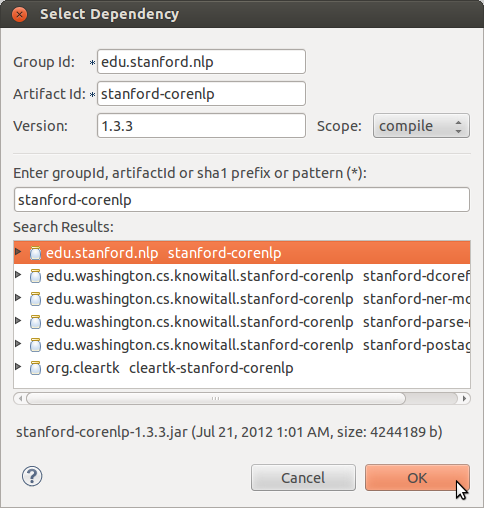
\includegraphics[scale=0.3]{repo-06-corenlp}
\caption{Searching for CoreNLP\label{repo-06-corenlp}}
\end{figure}

\item In the popup window, directly type in ``stanford-corenlp'' in the search box under the message \textbf{Enter groupId, artifactId or sha1 prefix or pattern (*)}, and select \textbf{edu.stanford.nlp stanford-corenlp}. Now you will find the three fields at the top: \textbf{Group Id}, \textbf{Artifact Id}, and \textbf{Version} will be automatically filled with the correct information. Click \textbf{OK} to continue.

\begin{figure}[t]
\centering
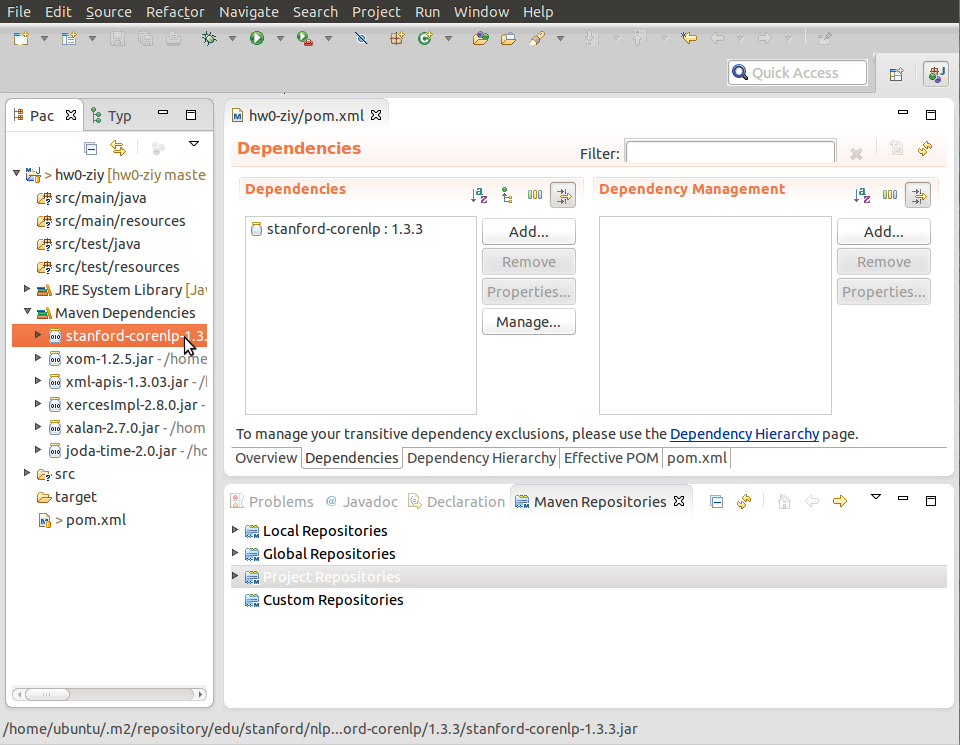
\includegraphics[scale=0.3]{repo-07-maven-dep}
\caption{Stanford CoreNLP appearing in Maven Dependencies\label{repo-07-maven-dep}}
\end{figure}

\item Finally, we could see the newly added dependency ``stanford-corenlp: 1.3.3'' is shown in the left column of ``Dependencies'' field. In addition, you will find the new dependency is also added to the Maven Repositories in the ``Project Explorer'' view. See Figure \ref{repo-07-maven-dep}.

\end{enumerate}

Now you have added the dependency on Stanford CoreNLP, and you will base on the denpendency to write in your own code in the next task.
